\documentclass[10pt, a4paper]{article}

\usepackage[a4paper, top=0.5cm, bottom=0.5cm, left=0.5cm, right=0.5cm, landscape]{geometry}
\usepackage{mathtools}
\usepackage{amsfonts}
\usepackage{multicol}
\usepackage{setspace}
\usepackage{graphicx}
\usepackage[dvipsnames]{xcolor}
\usepackage{array}



\author{Zachary Chua Yan Ern}
\date{February 2022}
\setstretch{1.25}

\newcommand{\highlight}[1]{{\color{red}\textbf{#1}}}
\newcommand{\blue}[1]{{\color{MidnightBlue}#1}}
\newcommand{\red}[1]{{\color{red}#1}}
\newcommand{\green}[1]{{\color{ForestGreen}#1}}
\newcommand{\header}[1]{{\normalsize\textbf{#1}}}
\newcommand{\tab}[0]{\hspace*{2mm}}

\begin{document}
	\scriptsize %tiny
	\setlength\parindent{0pt}
	\setlength{\columnseprule}{0.1pt}
	
	\begin{center}
		{\large CS3243 CheatSheet}\\
		by Zachary Chua
	\end{center}
	
	\begin{multicols*}{3}
	  \header{Agents and Environment}\\

	  \textbf{Agent Components}\\
	  Sensors and Actuators\\
	  - Sensors: information about the env\\
	  \tab - Percept data at timestep $t, p_{t}$\\
	  \tab - Percept History, $P = {p_{1}, ..., p_{t}}$\\
	  - Actuators: how agent interacts with environment\\
	  \tab set of \blue{Actions} $A$\\
	  \green{Agent function $f: P \rightarrow a$}, where $a$ is a selected action given $P$\\
	  Agent is rational if optimises performance measure (implies quantifiable objective), given\\
	  - percept seq\\
	  - prior knowledge\\
	  - set of actions\\
	  - performance measure\\
	  \highlight{Note:} do \textbf{not} assume agent is omniscient.\\

	  \textbf{Types of agents}\\
	  1. Reflex Agents\\
	  \tab - uses \texttt{if-else} to make decisions, direct mapping of percepts to actions\\
	  \tab - domain specific, impractical for large search space\\
	  2. Model-based reflex agent\\
	  \tab - makes decisions based on an internalised model\\
	  \tab - eg logical agents / bayesian networks\\
	  3. Goal \ Utility-based agents\\
	  \tab - Given \red{state, actions and goals / utility}\\
	  \tab - Determine \green{seq of actions} to reach goal / max utility\\
	  \tab - uninformed / informed search, Local Search, CSP, Adversarial Search\\

	  \textbf{AI as Graph Search}\\
	  - Each percept corresponds to a state in the problem (state $\rightarrow$ vertex)\\
	  - Define desired (goal) states\\
	  - After action, arrive at new state (actions are edges)\\
	  - Search space is graph\\

	  \textbf{Problem Env}\\

	  \begin{tabular}{ | m{1.5cm} | m{1.5cm} | m{5cm} | }
		\hline
		Fully observable & Partially observable & Whether can sense all information\\
		\hline
		Deterministic & Stochastic & Whether intermediate state can be determined based on action and state\\
		\hline
		Episodic & Sequential & episodic: action impacts current state, sequential: actions impact future states\\
		\hline
		Discrete & Continuous & for state information\\
		\hline
		Single & Multi agent & other entities that influence agent behaviour, competing or cooperating\\
		\hline
		Known & Unknown & Knowledge of agent (knowing where is goal state)\\
		\hline
		Static & Dynamic & If env will change while agent is deciding action\\
		\hline
	  \end{tabular}\\

	  \header{Path Planning}\\
	  \textbf{Properties}\\
	  Environment\\
	  \tab - Fully observable\\
	  \tab - Deterministic\\
	  \tab - Discrete\\
	  \tab - Episodic (plan solution, not execute, but plan is formed sequentially)\\

	  \textbf{Search Space}\\
	  State: representation of instance of environment\\
	  Node: Element in frontier representing current path traversed\\
	  \tab - State\\
	  \tab - Parent Node\\
	  \tab - Action\\
	  \tab - Path Cost\\
	  \tab - Depth\\
	  Goal Test function\\
	  Actions function\\
	  Action costs function ($\geq 0$)\\
	  Transition Model function: takes in a state, applies action, returns new state\\

	  \textbf{Algo Criteria}\\
	  Efficiency - space and time\\
	  \green{Complete} - find a solution when one exists and correctly report failure when it does not\\
	  \green{Optimal} - solution with \blue{lowest} path cost among all solutions\\

	  \textbf{Types of search}\\
	  Tree Search\\
	  \tab - No restrictions on revisiting states, allows redundant paths, including cycles\\
	  \tab - Incomplete, if there are cycles\\
	  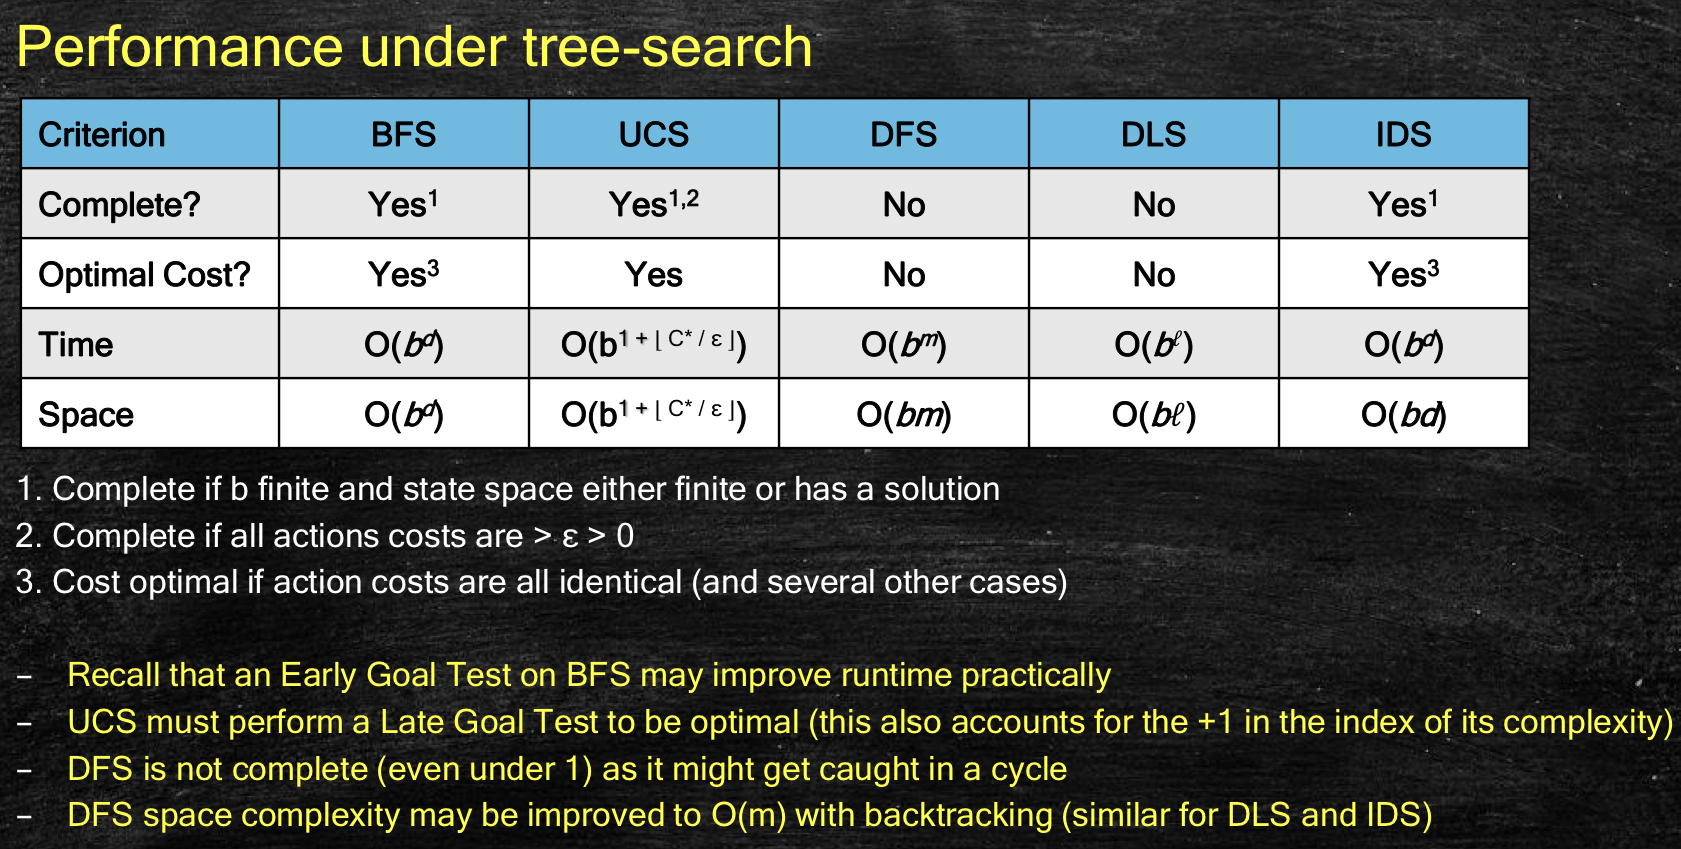
\includegraphics[scale=0.15]{./assets/treeSearch.png}\\
	  Graph Search\\
	  \tab - Maintain \texttt{reached} hash table \\
	  \tab - Add nodes to \texttt{reached} hash table on push\\
	  \tab - Only add new node to frontier (and \texttt{reached}) if\\
	  \tab \tab 1. state represented has not been reached before\\
	  \tab \tab 2. path to state already reached is cheaper than the stored one\\
	  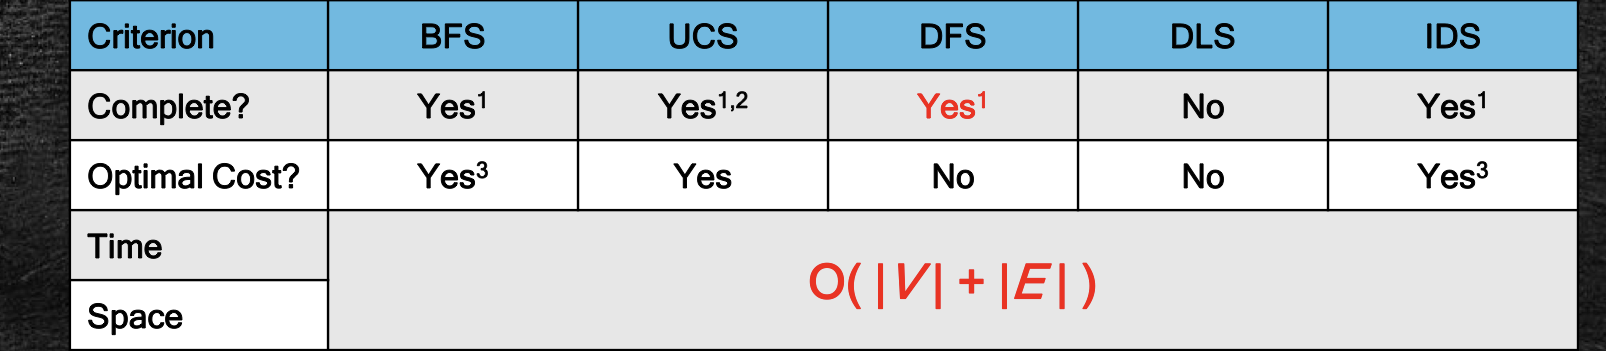
\includegraphics[scale=.15]{./assets/graphSearch.png}\\
	  Limited Graph Search V1\\
	  \tab - Uses \texttt{reached} hash table\\
	  \tab - Adds to \texttt{reached} on push to frontier\\
	  \tab - Only pushes to frontier when not in \texttt{reached}\\
	  Limited Graph Search V2\\
	  \tab - Similar to V1\\
	  \tab - Adds notes to \texttt{reached} on pop from frontier\\
	  \tab - \red{Does not} check if path is cheaper than stored one\\
	  \tab - \red{Not optimal} for UCS or A*\\

	  \header{Uninformed Search} \\
	  \textbf{BFS - Queue}\\
	  Time: $O(b^{d})$\\
	  Space: $O(b^{d})$\\
	  Complete: Yes if finite search space or contains solution\\
	  Optimal: No unless costs uniform\\
	  $b$: branching factor\\
	  $d$: depth of shallowest goal\\
	  \green{Can be optimised} with \red{early goal test} (goal test on push to frontier instead of pop)\\

	  \textbf{UCS aka Dijkstra - PQ, path cost}\\
	  Time: $O(b^{e})$ \\
	  Space: $O(b^{e})$\\
	  Complete: Yes if finite search space or contains solution\\
	  Optimal: Yes, tree, graph and limited V2\\
	  $e$: $1 + \lfloor \frac{C*}{\epsilon} \rfloor$, where C* is the optimal path cost\\
	  $\epsilon$: small positive constant, smallest action cost\\

	  \textbf{DFS - Stack}\\
	  Time: $O(b^{m})$\\
	  Space: $O(bm)$\\
	  Complete: No, unless finite search space\\
	  Optimal: No\\
	  $m$: max depth\\
	  \red{Note}: space can be improved to $O(m)$ by using backtracking (assume fixed order of actions)\\

	  \textbf{Depth Limited Search (DLS)}\\
	  DFS with depth limit $l$\\
	  Time: $O(b^{l})$\\
	  Space: $O(bl)$\\
	  Complete / Optimal: No\\

	  \textbf{Iterative Deepening Search (IDS)}\\
	  Use DLS recursively, each time increasing $l$ by 1\\
	  \tab - Completeness of BFS with space complexity of DFS\\
	  Overhead: rerun top levels many times ($\sim11\%$)\\
	  \tab - Nodes generated by DLS: $O(b^{0} + b^{1} + ... + b^{l})$\\
	  \tab - Nodes generated by IDS: $O((d + 1)b^{0} + db^{1} + ... + b^{d})$\\
	  Time: $O(b^{d})$\\
	  Space: $O(bd)$\\
	  Complete: same as BFS\\
	  Optimal: same as BFS\\

	  \header{Informed Search}\\
	  Use domain knowledge to estimate cost from $s$ to $G$ using heuristic function $h$\\
	  Define \red{evaluation function} $f$ to be used as priority function in PQ\\
	  UCS: $f = g$\\
	  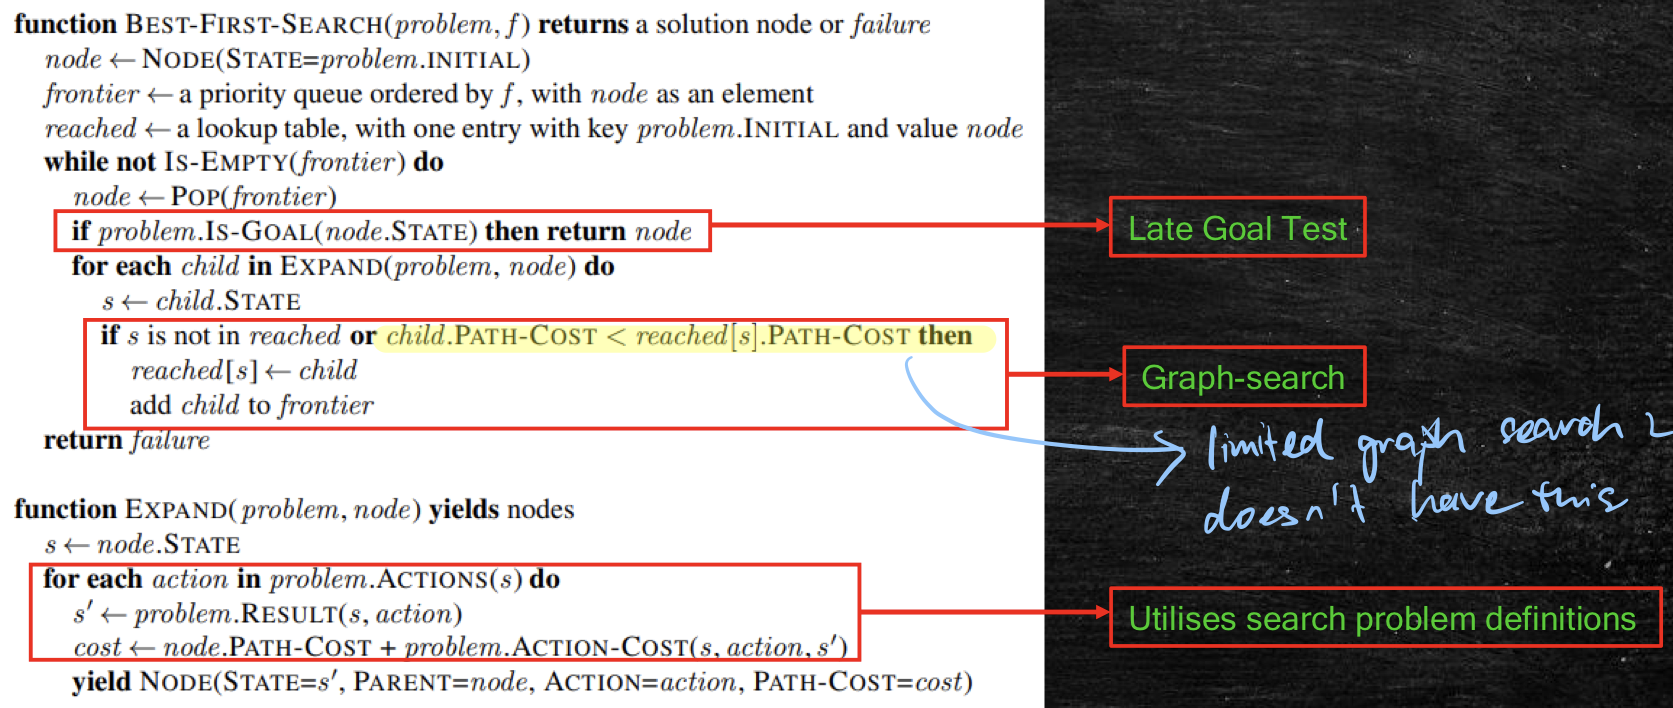
\includegraphics[scale=.16]{./assets/bestFirst.png}

	  \textbf{Greedy Best First Search}\\
	  Explore state that you estimate is closest to a goal\\
	  Evaluation fn: \green{$f(n) = h(n)$}\\
	  Optimal: \red{not optimal} as does not take into consideration cost of path travelled (one node very close to goal but high cost to get to adjacent to start node)\\
	  Tree Search: \red{Incomplete}, stuck between 2 nodes with lowest $h$ values\\
	  Graph Search: \red{Complete}, if search space is finite\\

	  \textbf{A* Search}\\
	  Evaluation fn: \green{$f(n) = g(n) + h(n)$}\\
	  Optimality:\\
	  \tab Admissible heuristic: Tree Search, Graph Search\\
	  \tab Consistent heursitic: Tree, Graph, Limited Graph V2\\
	  A* and Graph Search \red{costly} due to updates (need update descendants)\\

	  \header{Heuristics}\\
	  \textbf{Admissible Heuristics}\\
	  $\forall n, h(n) \leq h^{*}(n)$\\
	  \tab - $h(n)$ never overestimates the cost\\
	  \tab - $h(n) = 0$ at goal\\

	  \textbf{Consistent Heuristics}\\
	  $\forall n, n', h(n) \leq cost(n, a, n') + h(n')$\\
	  \tab - $f$ costs monotonically increasing along a path\\

	  \textbf{Dominance}\\
	  if $\forall n, h_{1}(n) \geq h_{2}(n)$, then $h_{1}$ dominates $h_{2}$\\
	  - if $h_{1}$ is also admissible: $h_{1}$ \green{closer} to $h^{*}$, $h_{1}$ more \green{efficient} than $h_{2}$\\
	  \highlight{Note}: for 3243, $h_{1}$ and $h_{2}$ need not be admissible\\

	  \textbf{Creating heuristics}\\
	  - Want \green{efficient} $h$, close to $O(1)$\\
	  - Want \green{admissible}, consistent harder\\
	  \textbf{Relaxing the problem}\\
	  \tab - relaxing constraints gives admissible heuristics\\
	  \tab - relaxing more constraints creates \red{less} dominant heuristics\\
	  \textbf{Top Down Approach}\\
	  - What dependent variable do I want to model / approx\\
	  - What are the independent variables that help to calculate these\\
	  \textbf{Bottom up Approach}\\
	  - What variables can you efficiently calculate?\\
	  - What can these variables model?\\

	  \header{Local Search Problems}\\
	  - Only have goal test, but not values in goal state\\
	  - Want goal state values, not interested in path\\
	  - Greedy \red{not} systematic\\
	  - Space Complexity: $O(b)$, only store node and successors\\

	  \textbf{State formulation}\\
	  - All states have all components of solution\\
	  \tab - no partially filled states\\
	  - Each state is a potential solution\\
	  \tab - ``guess'' a soltion\\
	  \tab - ``check'' its value\\
	  \tab - make ``systematic guess'' by moving to states of higher value (higher value closer to goal)\\

	  \textbf{Steepest Ascent Hill Climbing Algorithm}\\
	  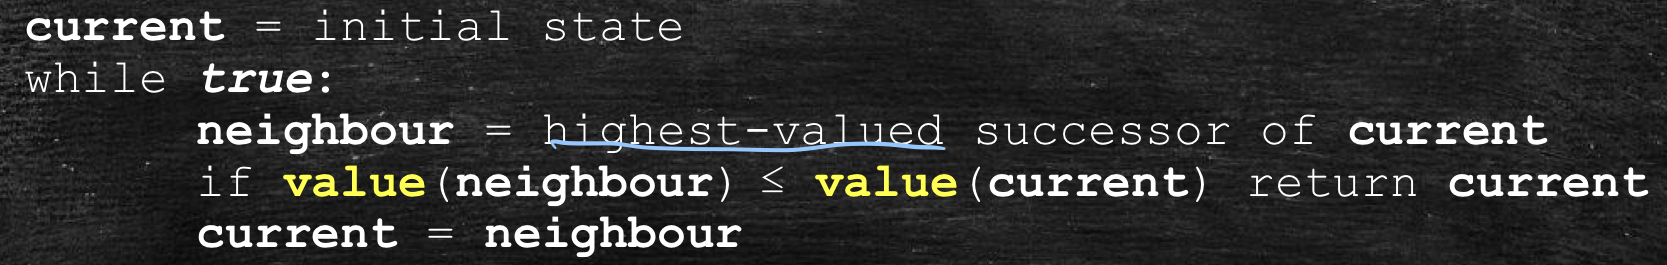
\includegraphics[scale=0.15]{./assets/steepestAscent.jpeg}\\
	  - Only store current state\\
	  - On each iteration, find successor that \textbf{improves} on current state\\
	  \tab - Requires \red{\texttt{actions}} and \red{\texttt{transitions}} to determine successor\\
	  \tab - Requires \red{\texttt{value}}: a way to assign each state a value ($f(n) = -h(n)$)\\
	  - If none exists, return current state as the bes option\\
	  \tab - \highlight{Can fail}, may reutrn non-goal state\\
	  \tab - may fail at \red{local maxima, shouldder \ plateau, ridge}\\

	  \textbf{Variants}\\
	  - Sideways move: replace $\leq$ with $<$\\
	  \tab - \green{Can traverse shoulder}\\
	  - Stochastic hill climbing: chooses randomly among states with values better than current\\
	  \tab -\green{ try to prevent getting stuck at local maxima }\\
	  - First Choice: handles \red{high $b$} by randonly generating successors and choosing first one that is better\\
	  \tab - \green{Similar to stochastic, handles high $b$}\\
	  - Random restart: add outer loop which randomly picks new start state until solution found\\
	  \tab - \green{Guaranteed to find solution}\\

	  \textbf{Analysis}\\
	  let $p_{1}$ be probability of success, $n_{1}$ be number of steps of expected solution, $n_{2}$ be no. of steps of expected failure\\
	  \centerline{Expected Computation = $n_{1} + \frac{1 - p_{1}}{p_{1}} * n_{2}$}\\

	  \textbf{Local Beam Search}\\
	  Algo:\\
	  1. Begin with $k$ random starts\\
	  2. Each iteration generate successors for \red{all} $k$ states\\
	  3. Repeat with best $k$ among \red{all} successors unless goal found\\
	  Better than k parallel random restarts $\rightarrow$ best $k$ among \highlight{all} successors, not best from each set of successors, $k$ times\\
	  \textbf{Stochastic Beam Search}\\
	  Similar to stochastic hill climbing\\

	  \header{Constraint Satisfaction Problem}\\
	  Systematic search unlike LSP greedy search\\
	  \textbf{Formulating CSP}\\
	  State Representation:\\
	  - Variables: $X = {x_{1}, x_{2}, ... , x_{n}}$\\
	  - Domains: $D = {d_{1}, d_{2}, ... , d_{n}}$\\
	  \tab - such that $x_{i}$ has domain $d_{i}$\\
	  - Initial State: all variables unassigned\\
	  - Intermediate State: partial assignment\\
	  Goal Test\\
	  - Constraints: $C = {c_{1}, c_{2}, ... , c_{m}}$\\
	  - Each $c_{i}$ describes necessary relationship $rel$, between set of variables $scope$\\
	  \tab - eg. $scope = (x_{1}, x_{2})$ and $rel = x_{1} > x_{2}$\\
	  - constraints can be \red{unary, binary, global}\\
	  Actions and Transitions\\
	  - costs and evaluation function not utilised\\

	  Objective: find \green{complete} and \green{consistent} assignment\\
	  - complete: all variables assigned\\
	  - consistent: all constraints in $C$ satisfied\\

	  \textbf{CSP search algo}\\
	  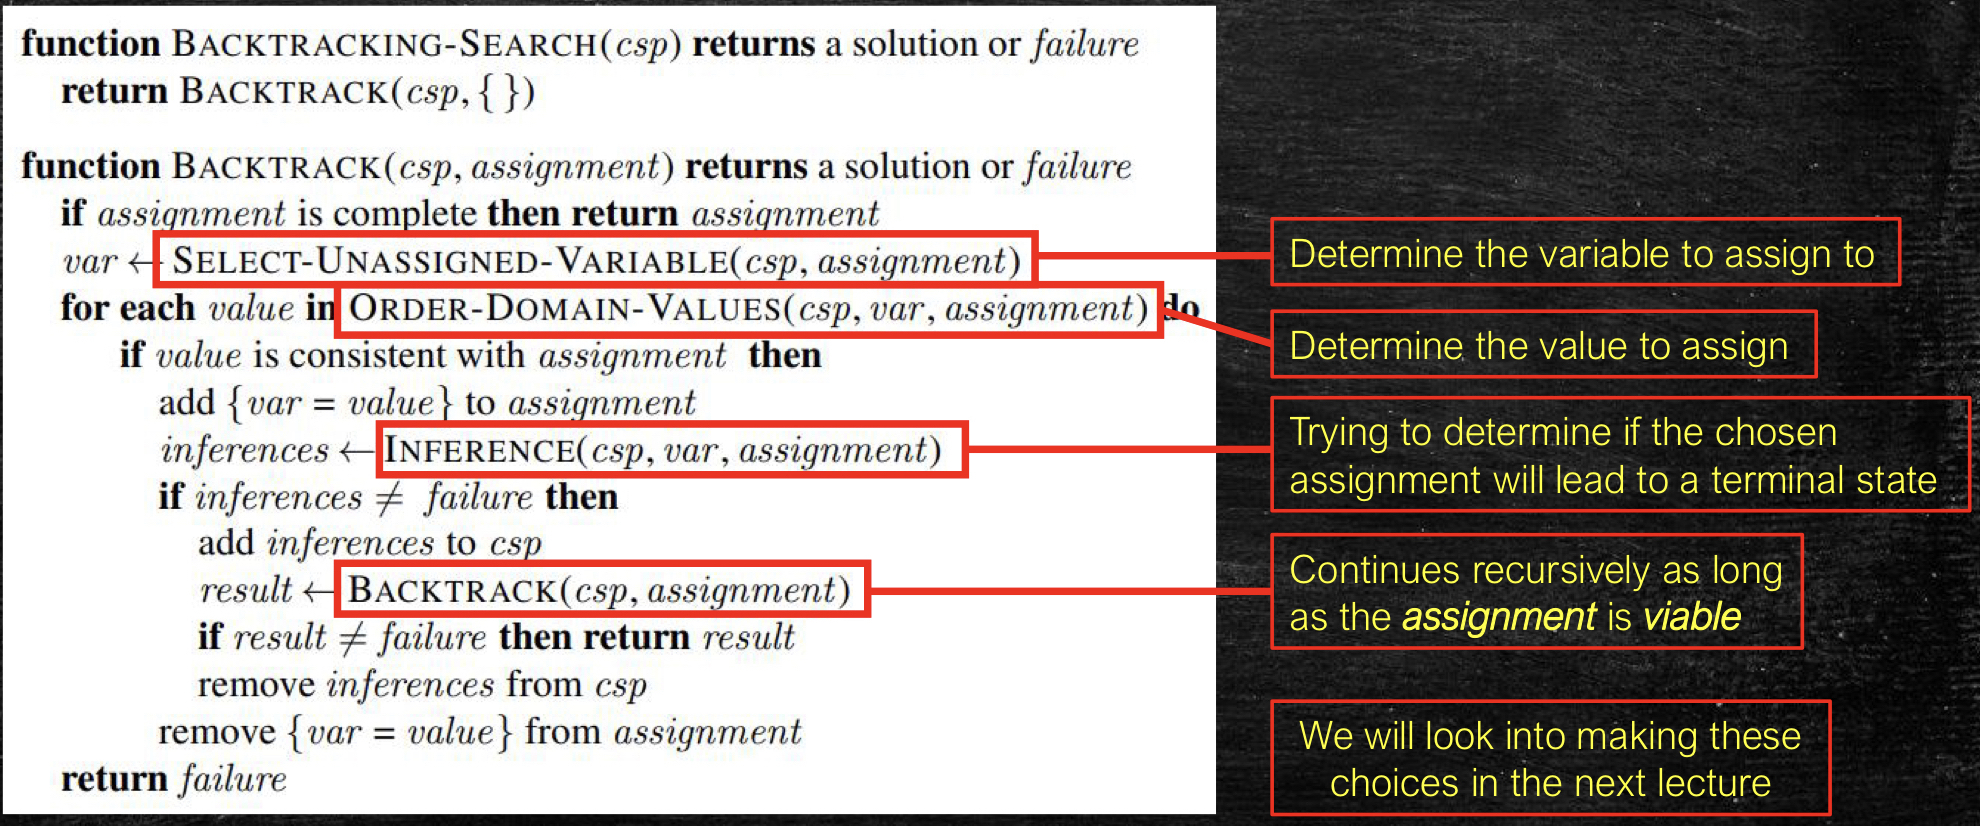
\includegraphics[scale=0.135]{./assets/CspBacktracking.jpeg}\\
	  - Use DFS as solutions \green{are all at} max depth\\
	  - Each level assign to only \green{one variable}, \red{not all} because order does not matter (prunes tree)\\
	  - Backtrack when there are no legal assignments\\

	  









	\end{multicols*}
\end{document}
